\section{Correlation between Submission Properties and Detection Rate}
\label{sec:corr}
This section presents our study of the correlation between various properties of \pe\ submissions and the detection rate of \pe\ submissions.
Detection rate is what most \vt\ users use to decide whether their submissions are benign or malware 
and the first thing that a user of \vt\ uses.
Therefore, it is important to study what factors affects or correlates to detection rate
and the results can guide security researchers and vendors to have targeted investigation over {\em suspicious} files, 
files that have the factors that we identify as highly correlated to detection rate.

We studied a range of properties and their correlation with detection rate
and found that three factors have higher correlation:
submission file size,
historical submission properties, and the reputation of source IDs.
We present these correlation study results in this section.
In the next section, we will present our further analysis of what can affect the detection result of anti-virus engines
and if detection rate is a perfect measurement of the likelihood of malware.

\begin{figure}[t!]
\begin{center}
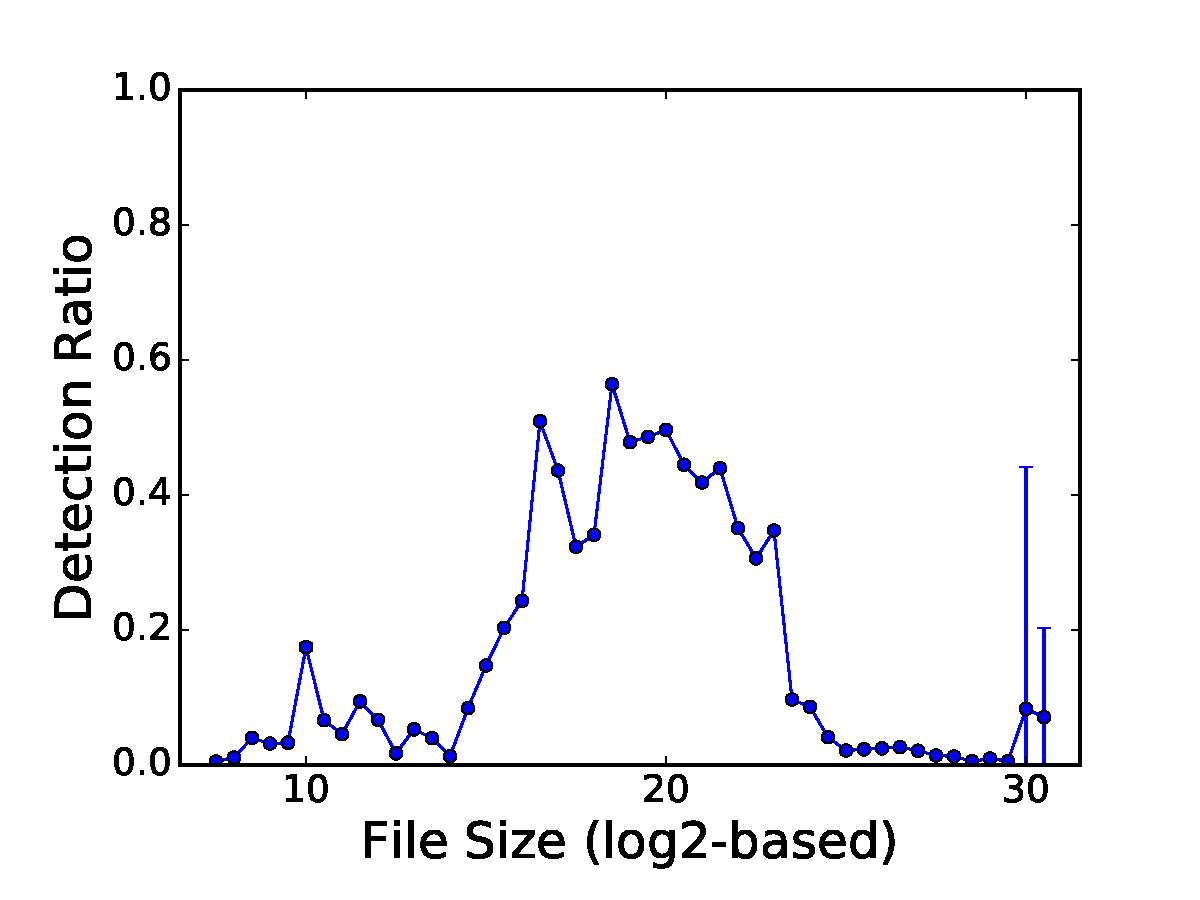
\includegraphics[width=2in]{figure/size}
  \caption{How detection rate changes with file size.
(
95\% confidence interval is also drawn for each point.
Results of log2 for the original file sizes are rounded to the nearest 0.5 value.)
}
\label{fig:size}
\end{center}
%\vspace{-0.25in}
\end{figure}


\subsection{File Size}
\label{sec:size}
Anecdotally, \pe\ malwares are most likely to have small to medium size. 
To verify this, we analyzed the relationship between submission file size and detection rate. 
Figure~\ref{fig:size} presents the average detection rate and 
the 95\% confidence interval for different file sizes.
A wider confidence interval implies that
the calculated average detection rate is farther away from the real average detection rate.
We use discrete file sizes of powers of two in our analysis and in this graph,
i.e., we calculate the log2 of each original file size and round it to the nearest 0.5 value.
Overall, we find that files with size from 90KB to 4MB have higher detection rate, more than 20\% on average. 
Except for the last two points which represent a small amount of files that are bigger than 1GB, 
all other sizes have high confidence.   

{\bf Observation 4:} 
{\em \pe\ malwares are mostly likely to have small to medium size.}

An immediate question to raise is whether the high detection rate of files with small to medium size
is because these files also contribute to most of the submissions as shown in Figure~\ref{fig:pesize}.
As we will discuss in Section~\ref{sec:history}, the correlation of submissions and detection rate is more complex and non-linear.
Thus, there is a more fundamental reason behind the file size correlation with detection rate.
One likely reason of this correlation is that files that are too small are not enough to express the
malware functions while files that are too big are difficult to spread.

\subsection{Submission History}
\label{sec:history}

%\begin{figure*}[!htb]
\minipage{0.31\textwidth}
  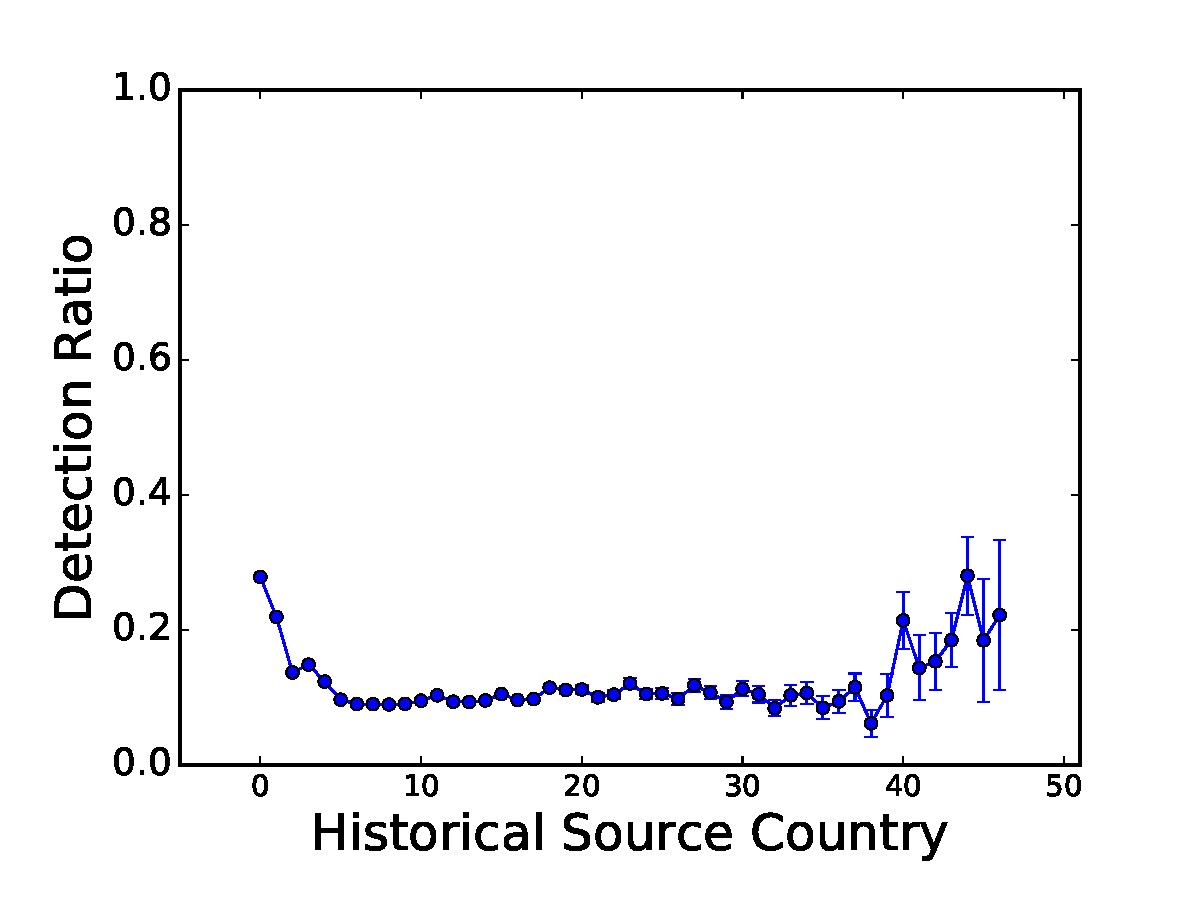
\includegraphics[width=\linewidth]{figure/SubCountry}
  \mycaption{fig:hiscountry}{The relation between the number of historical source countries and detection rate.}
{\footnotesize{(How detection rate changes with the number of historical source countries.
95\% confidence interval is also drawn for each point.)}}
\endminipage\hfill
\minipage{0.31\textwidth}
  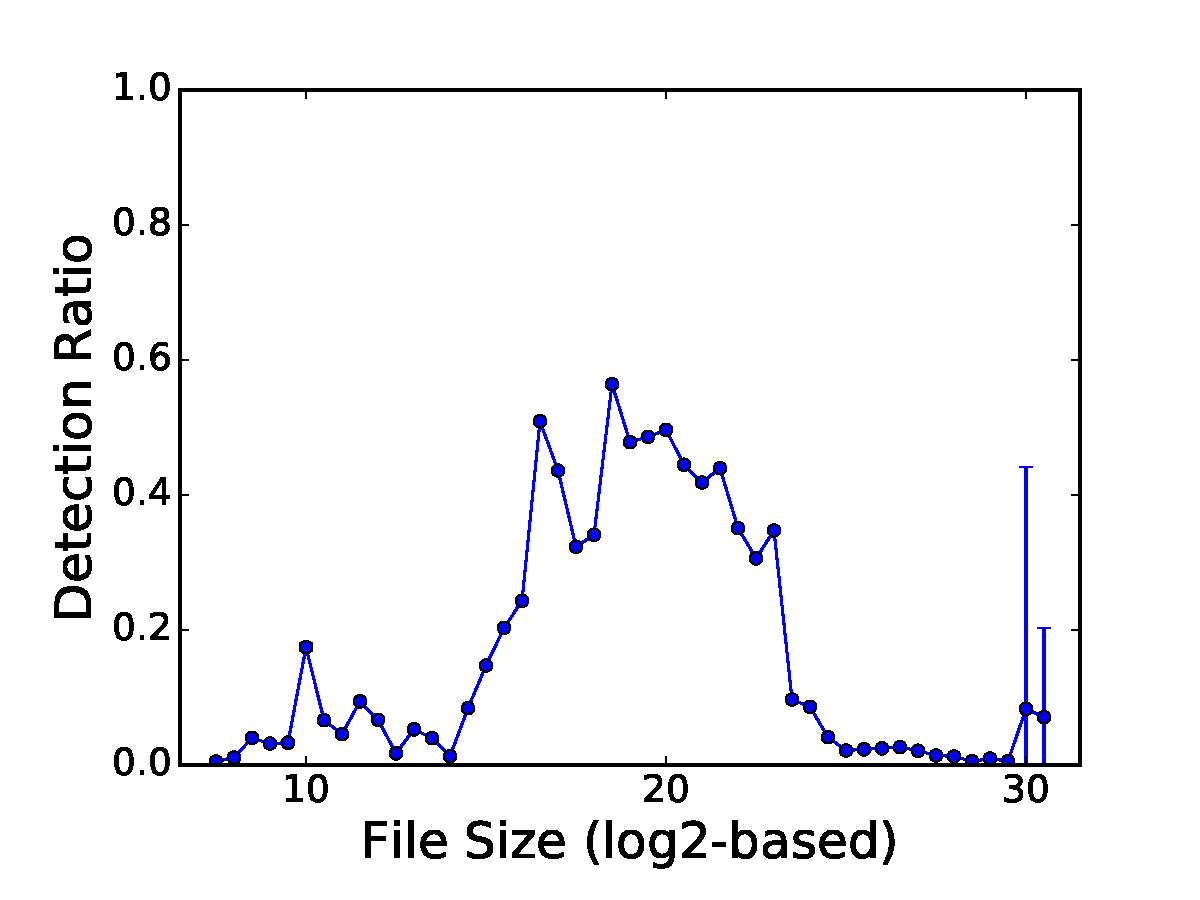
\includegraphics[width=\linewidth]{figure/size}
  \mycaption{fig:size}{How detection rate changes with file size.}
  {\footnotesize{(How detection rate changes with log2-based file size.
Results from log2 are rounded up to nearest 0.5.
95\% confidence interval is also drawn for each point.)}}
\endminipage\hfill
\minipage{0.31\textwidth}%
  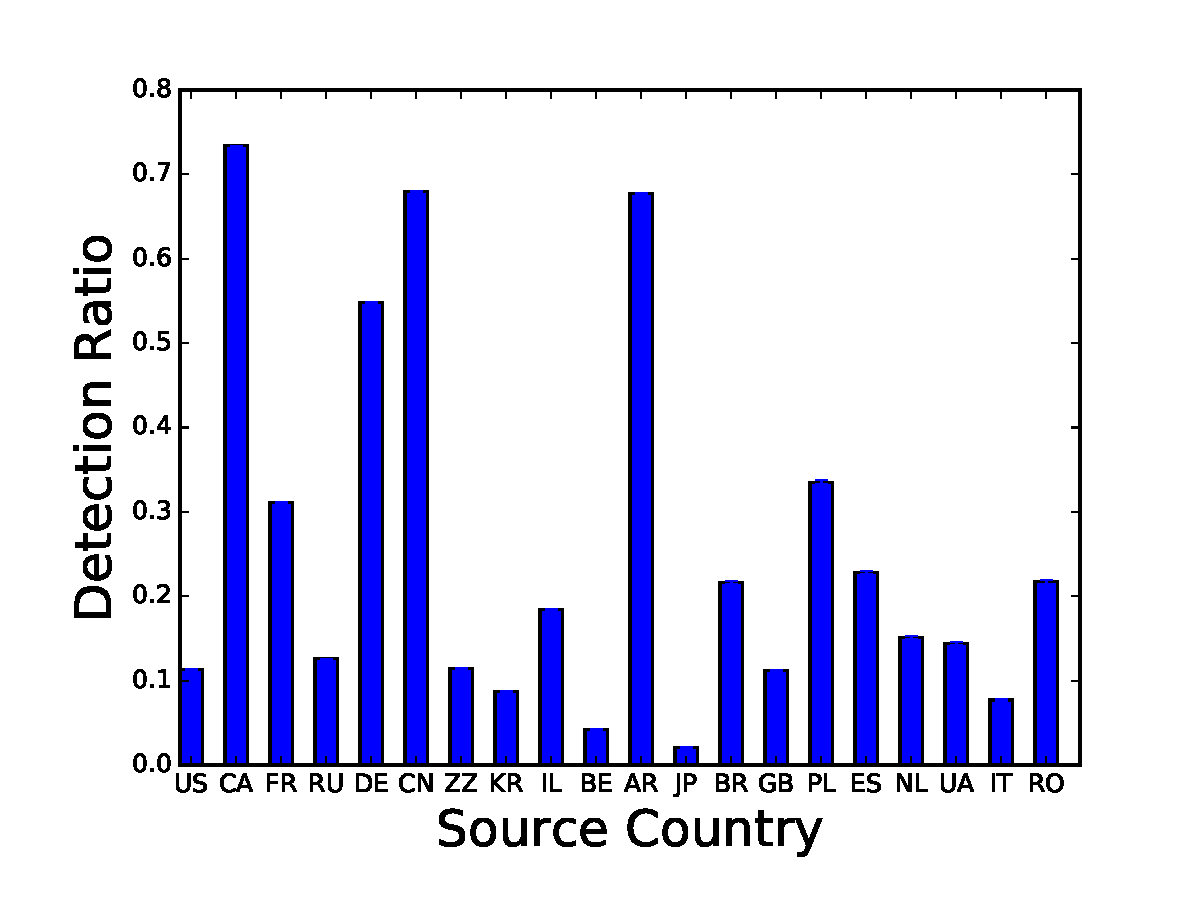
\includegraphics[width=\linewidth]{figure/Country}
  \mycaption{fig:Country}{Average detection rate for top 20 countries.}
{\footnotesize{(Average detection rate for submissions from countries ranking 
in top 20 in making PE submissions to VirusTotal. 
95\% confidence interval is also drawn for each country.)}}
  %\label{fig:aveUncover}
\endminipage\hfill

%\vspace{-0.2in}
\end{figure*}



\begin{figure}[t!]
\begin{center}
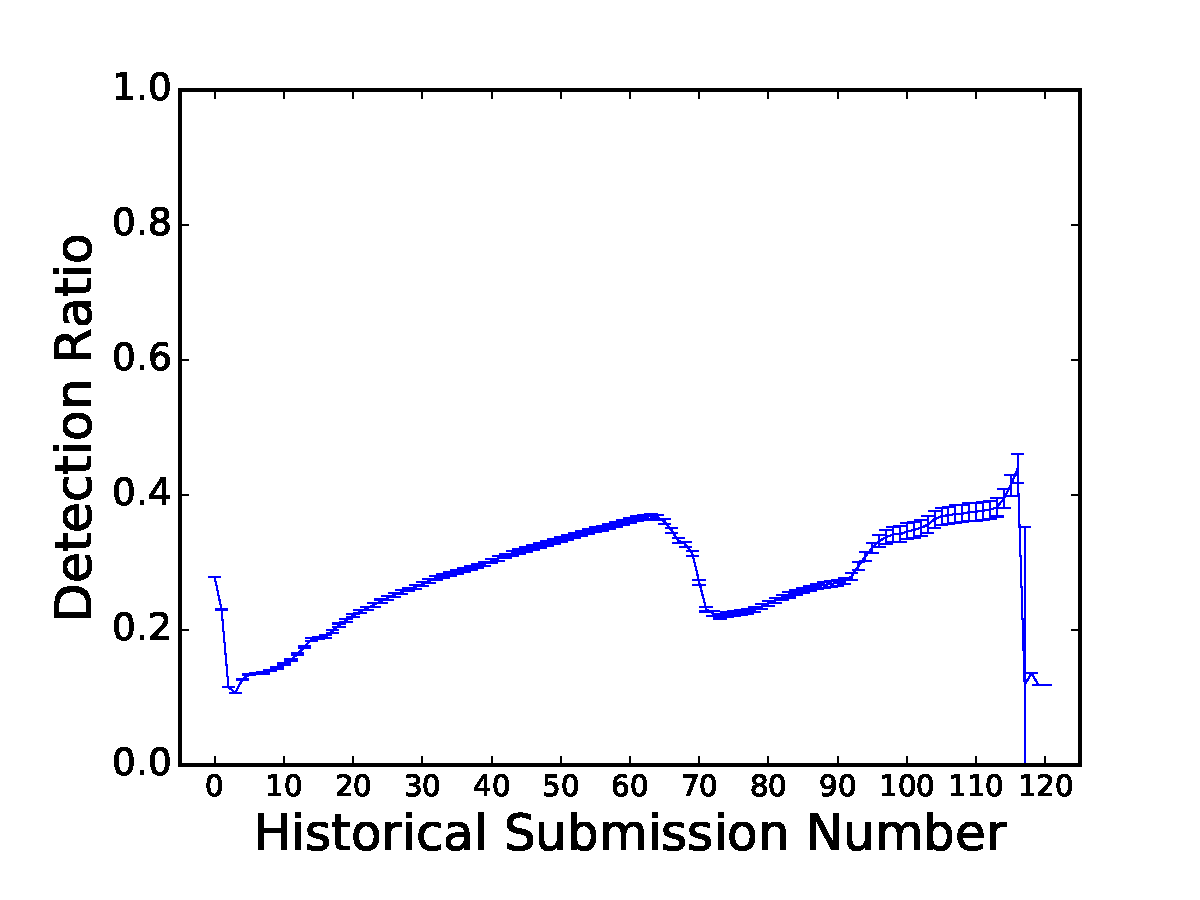
\includegraphics[width=2in]{figure/SubNum}
\caption{
The relation between historical submission number and detection rate.
(
How detection rate changes with historical submission number. 
Each historical submission number is rounded up to nearest 5.
95\% confidence interval is also drawn for each point.
)	
}
\label{fig:hisnum}
\end{center}
%\vspace{-0.25in}
\end{figure}

%\begin{figure}[t!]
%\begin{center}
%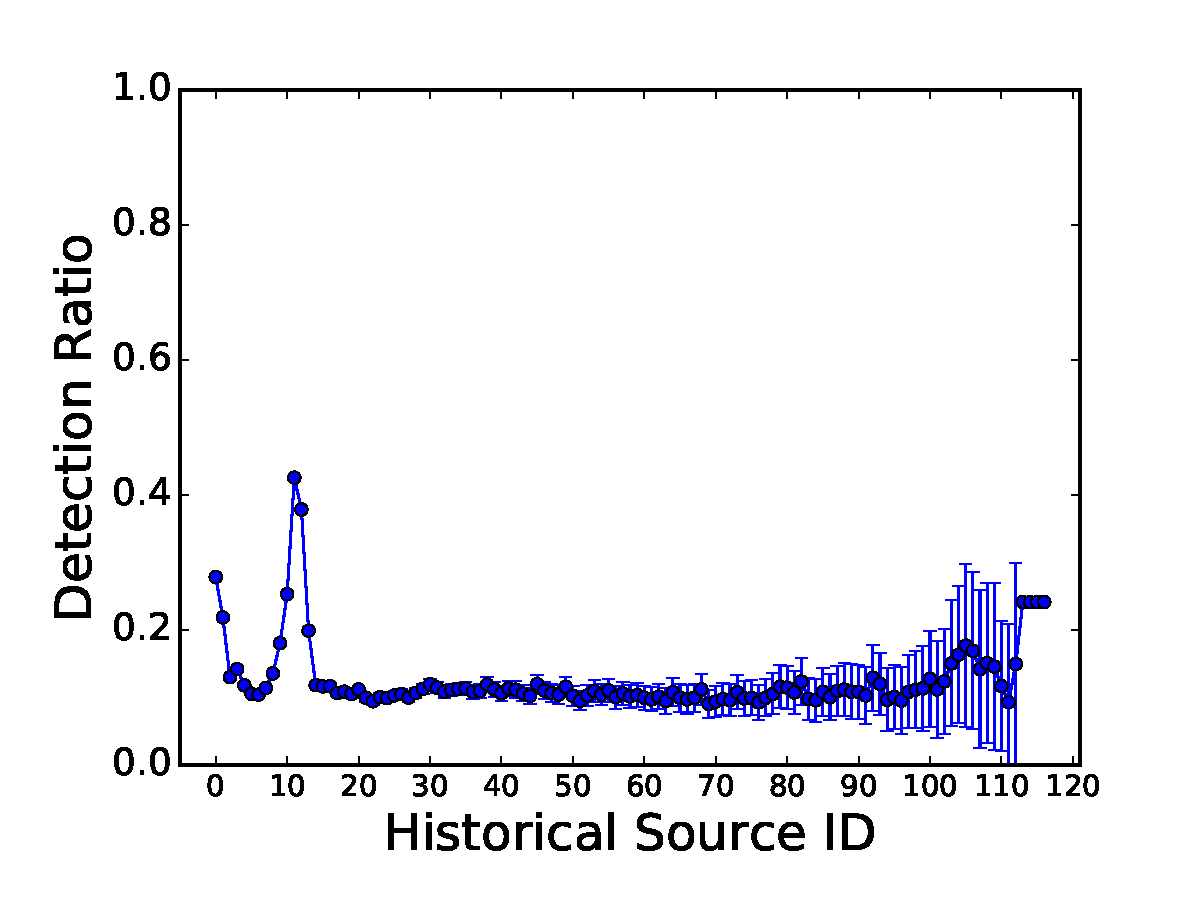
\includegraphics[width=2.5in]{figure/SubID}
%  \mycaption{fig:hisid}{The relation between the number of historical source ids and detection rate.}
%{\footnotesize{(How detection rate changes with the number of historical source ids. 
%Each historical number of source ids is rounded up to nearest 5.
%95\% confidence interval is also drawn for each point.)}}

%\end{center}
%\vspace{-0.25in}
%\end{figure}


As discussed in Section~\ref{sec:basicanal}, there are files that have been submitted more than once to VirusTotal. 
It is worthwhile to investigate this {\em history of submission} and how history affects future.
We study the correlation between submission history and the detection rate of the current submission.
Among the different types of historical information that we study,
we find that two types have higher correlation to detection rate:
the number of submissions made in history and the number of source IDs that made submissions of the same file in history.
%Given a submission, we also study whether information for historical 
%submissions of the same file influences detection rate for the current submission. 

%\noindent{\textit{\underline{The number of submissions in history.}}}
To study the submission history, we first sort all submissions for each file chronologically
and then collect the number of all submissions made before submission $s$ for each submission $s$ in \vt.
Next, we calculate the correlation between detection rate and the number of submission in history.
Figure~\ref{fig:hisnum} plots how detection rates change over the number of historical submissions.
Interestingly, there are two main ranges that steadily increase and there are three drops in the beginning, middle, and end.

To explain this effect, we first look at the two factors that can both influence detection rates:
the percentage of benign files submitted and the amount of anti-virus engines labeling the submission as malware.
%Two factors can influence detection rates and explain the above effect.
Obviously, with more benign files submitted, detection rate will decrease.   
and with more engines labeling malwares, detection rate will increase. 
In the the two stages of detection rate increasing, 
with more submissions, more engines are able to identify malwares 
and the increase of percentage of engines identifying submitted malwares dominates. 
In the range that detection rate drops, 
VirusTotal users stop submitting files that have already been identified as malwares,
and the increase of percentage of benign files submitted to VirusTotal dominates. 

%\noindent{\textit{\underline{Number of submitted source IDs in history.}}}
%One file can be submitted by one source ID multiple times 
%and can also be submitted by different source IDs multiple times. 
%We now study the correlation between the number of source IDs in the submission history and the detection rate. 

%\yiying{the whole explanation for this figure needs to be filled here.}
%Figure~\ref{fig:hisid} plots the detection rate and confidence interval as the number of historical source IDs increases. 
%Confidence intervals increases when there are more than 50 source IDs. 
%Detection rate is higher for historical source IDs less than 12, compared with historical source IDs more than 12.
%{\color{red} The X for the largest point is 11. }
%\yiying{is it 12? I cannot tell for sure by just looking at the figure}
%The number of historical source IDs reflects the popularity of a submitted file.
%When the popularity of a file is larger than a certain value, 12 for our dataset, 
%file popularity is unrelated to detection rate. 
%{\color{red} When a file is submitted more than certain number of users, or popular than centain threshold, 
%it is likely to be thoroughly analyzed by all engines, and all vendors have made their decision. 
%They either consider the file as malware or not. They will not change decision. }
%\yiying{why?}

{\bf Observation 5:} 
{\em  When historical numbers fall into certain range, they are correlated with detection rate.}

\if 0
\noindent{\textit{\underline{Historical source country.}}}
One file could also be submitted from different countries. 
The number of historical source countries also reflect the popularity of a submitted file. 
The correlation between detection rate and the number of historical source countries in 
Figure~\ref{fig:hiscountry} shows similar trend as the correlation between detection rate 
and the number of historical source IDs in Figure~\ref{fig:hiscountry}. 

Figure~\ref{fig:hisnum}, Figure~\ref{fig:hisid}, and Figure~\ref{fig:hiscountry} show that 
when historical numbers fall into certain range, they are correlated with detection rate. 
\fi

\subsection{Reputation of Source ID}
\label{sec:reputation}



\begin{figure}[t!]
\begin{center}
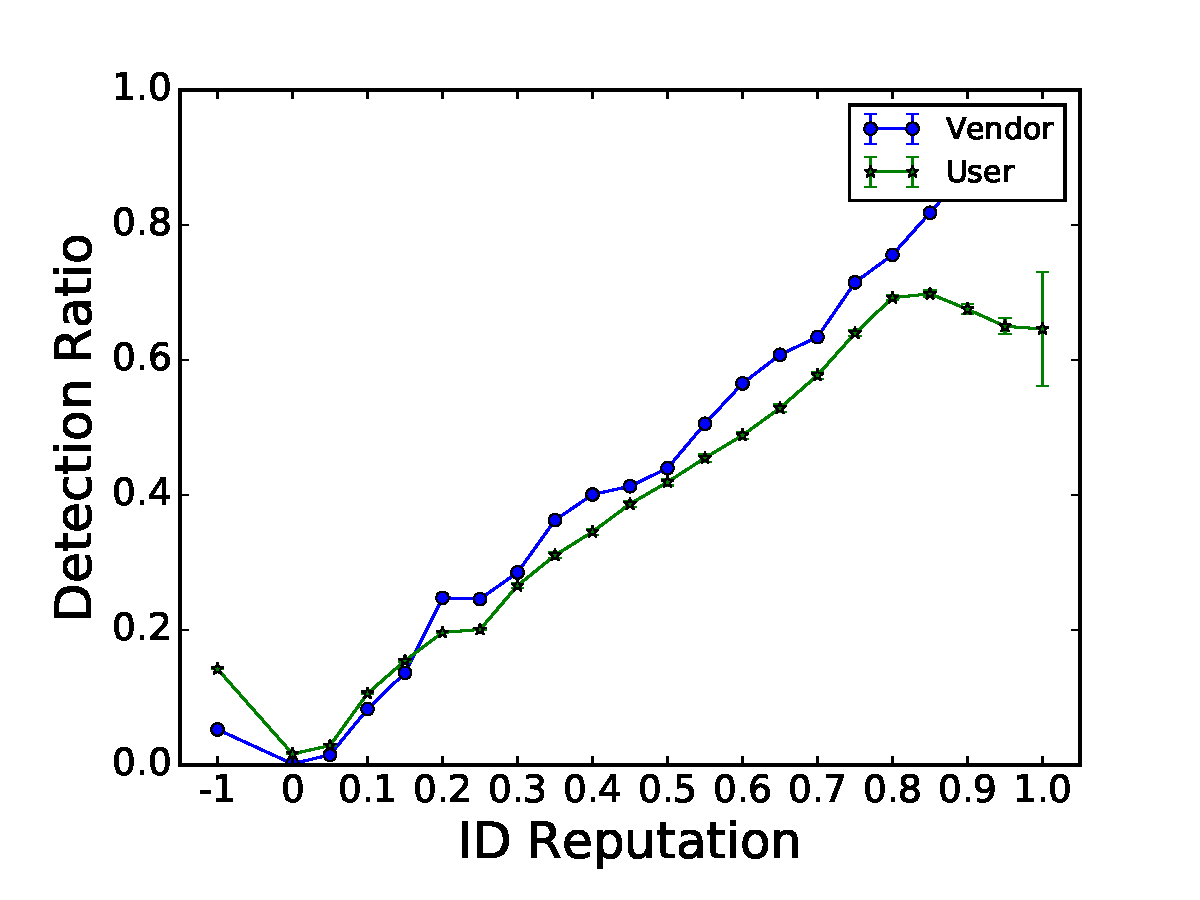
\includegraphics[width=2in]{figure/IDReputation}
\caption{The relation between source id's previous reputation and detection rate.
(How detection rate changes with the value of source id's reputation. 
Each reputation is rounded up to nearest 0.05.
Reputation -1 means the source id did not make any submission before. 
95\% confidence interval is also drawn 
for each point.)
}
\label{fig:idreputation}
\end{center}
%\vspace{-0.25in}
\end{figure}

Different users of online services such as \vt\ often have different {\em reputation} 
because of different motivations, objectives, and backgrounds.
For example, some users can randomly trying out \vt\ with no specific objective and thus submit random files
while other users have clear goals and motivations and thus only submit suspicious files.
The rationale behind reputation is that \vt{} users would have a roughly constant submission pattern, 
and it is promising to use their historical submission to predict their future submission.
Previous work~\cite{GuoICSE2010} reported that there is a correlation between bug reporter’s reputation and the likelihood for the bug being fixed. 
We also observe correlation between the reputation of source ID and submission’s detection rate. 

Intuitively, a user that have submitted more files that were detected as malware suggest 
that she is more likely to use \vt\ to detect malwares in suspicious files 
and thus should be given higher reputation.
To quantify this, we define the reputation of a source ID as the follow.
The reputation of a source ID is not a fixed value and can change over time. 

%\theoremstyle{definition}
\begin{definition}{Reputation:}
Given a submission $S$ with source ID $N$, 
we define the reputation of $N$ when conducting the submission $S$ as the average detection rate for all submissions conducted by $N$ before $S$. 
If $N$ did not make any submission before, we define the reputation to be $-1$. 
\end{definition}

Before conducting our source ID reputation analysis, we first filter out submissions without source ID information (for a small amount of submissions, \vt\ fails to provide source ID),
files that are only submitted once, and files that are submitted more than 1 million times (bogus or robots).
%For around 14\% PE submissions, VirusTotal fails to provide source ID information. 
%We filter out these submissions, when computing reputation.
%All other PE submissions are conducted by 613 thousand source IDs. 
%66\% source IDs only conduct submission once. 
%We filter source IDs conducting more than 1 million PE submissions in our data set, 
%because we think these are anti-virus vendors routinely test their products. 
To calculate source ID reputation, we first sort all submissions from the same source ID chronologically, 
and calculate reputation for each source id when conducting each submission. 
We further separate normal users from vendors and analyze the correlation of their ID reputation and detection rate.

Figure~\ref{fig:idreputation} plots the average detection rate and the 95\% confidence interval 
as the source ID reputation increases for normal users and for anti-virus vendors.
We round up reputation values to their nearest 0.05 values. 

Detection rate steadily increase as the reputation increases from 0 to 1 for vendors and from 0 to 0.8 for normal users.
Except the points when reputation is 1, all other results have high confidence.
Interestingly, for both normal user and vendors the detection rate with reputation -1 is higher than with reputation 0,
which means that the first submissions conducted by all source IDs (reputation -1) 
are overall have higher detection rate than 
the submissions conducted by IDs that have only submitted benign files (reputation 0).

For normal users, the detection rate drops when reputation is greater than 0.8.
This means that for normal users, it is difficult for them to always submit suspicious files detected by almost all vendors.
Vendors do not have this behavior and their detection rate always increases with higher reputation (other than reputation -1).


{\bf Observation 6:} 
{\em There is a high correlation between user reputation and detection rate of their submissions for both normal users and anti-virus vendors.}


\subsection{Discussion}

%\noindent{\textit{\underline{How to use our data?}}}
From our analysis, file size, number of submissions in history, and source ID reputation
are all highly correlated with detection rate. 
These results suggest that future researchers and vendors can use these values to have an initial estimation or prediction of future submissions.
Doing so can help reduce researchers' and vendors' effort to focus on more interesting files---files that are more likely to be malicious.
Anti-virus vendors can also inspect results which are variant from our studying results 
to identify possible false positives or false negatives in their products. 

%Linhai, it's not good to say things that you haven't done, esp. in a system paper. so I deleted the regression model discussion
%A possible future work is to train a regression model to combine all these factors together and 
%predict how many engines could detect a malware or how likely a file is a malware. 
%Using the regression model or our studying results alone, 
%security experts can prioritize malwares and focus their efforts on malwares which are more malicious. 
%Anti-virus vendors could inspect results which are variant from our studying results 
%to identify possible false positives or false negatives in their products. 


%In the future, we could design our reputation and historical metrics based on a tunable time windows, and investigate whether correlations still exist.   
